% !TEX root = ../main.tex


\section{Run To Completion}

The run to completion semantics is implemented via an abstract basis that is extend by the model. 
Figure~\ref{fig:basis} shows a statechart representation of how the basis enforces 
the run to completion semantics on the model transitions. 
\todo{Change r2c figure to make sure we have all necessary details. It is not clear right now. A legend may help}
\begin{figure}[!h]
	\vspace{-.4cm}
	\centering
	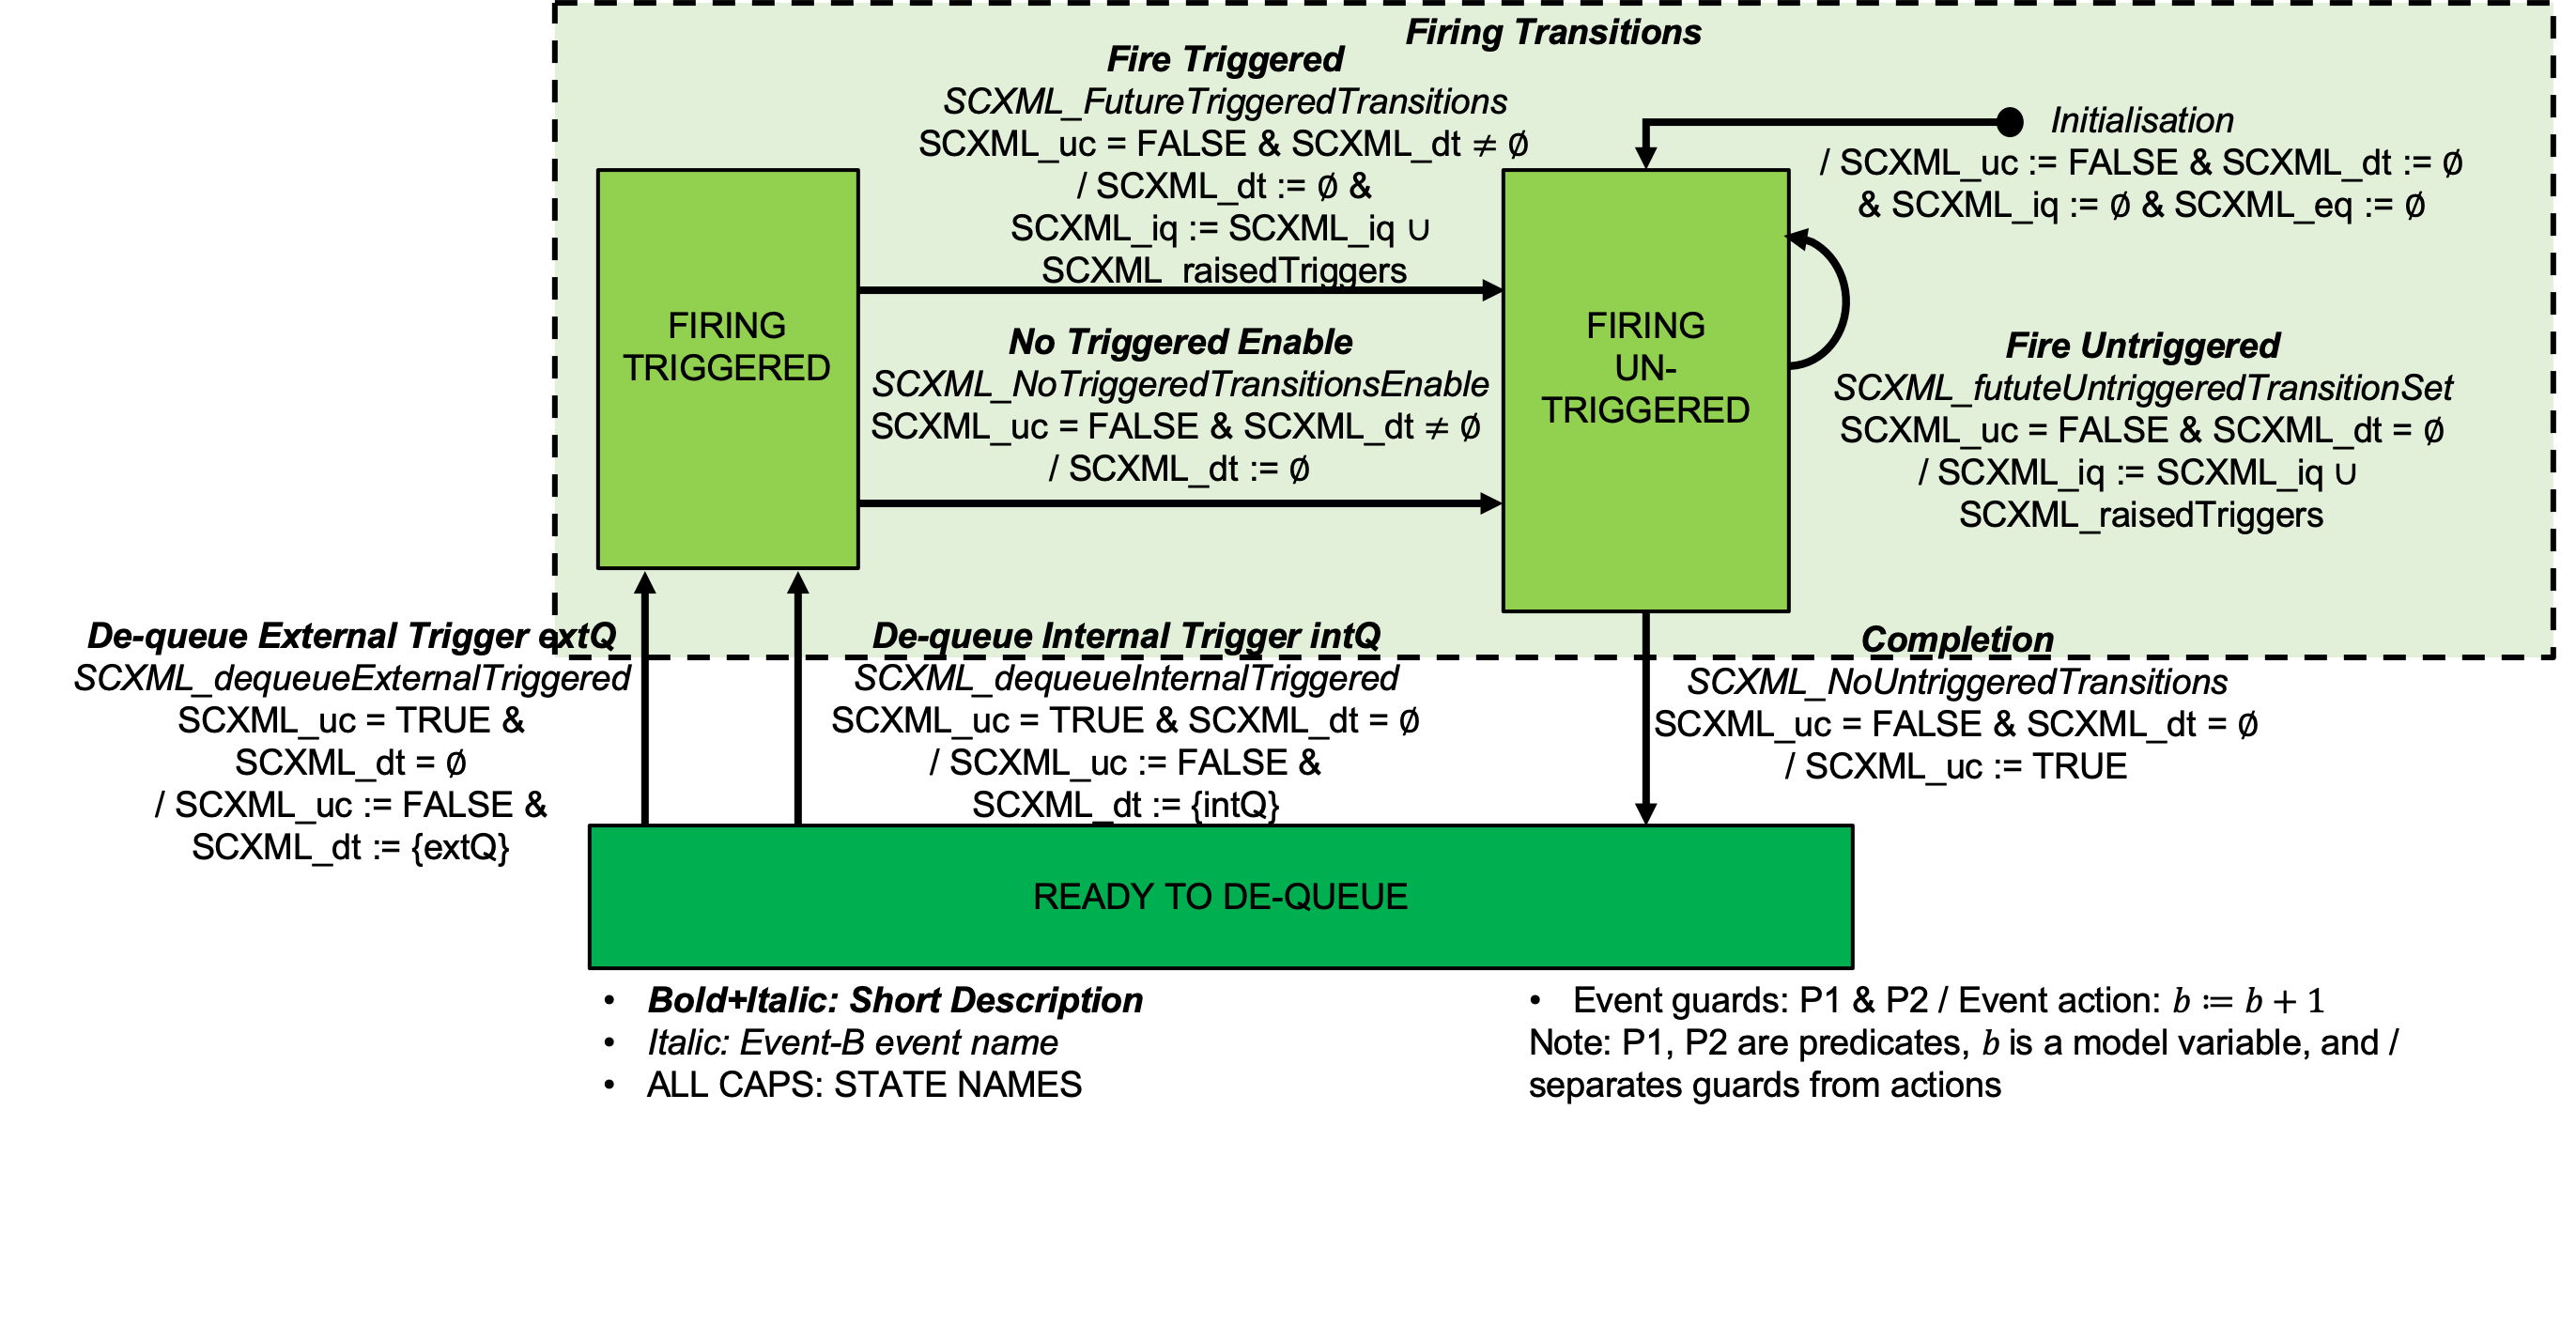
\includegraphics[width=0.99\textwidth, trim=0 100 0 0]{figures/Picture7.png}
	\caption{Abstract representation of run to completion basis}
	\label{fig:basis}
	\vspace{-.4cm}
\end{figure}

% The translation from \SCXML to \EVENTB is based on an abstract `basis' that models the `run to completion' semantics. 
The implementation of this basis consists of an \EVENTB \emph{context} and \emph{machine} that are 
the same for all input models and are refined by the specific output of the translation.  
% The basis context, Listing~\ref{lst:BasisContext}, introduces a given set of all 
The basis context introduces a given set of all 
possible triggers and is partitioned into internal and external ones, 
some of which will be introduced in future refinements. 
Refinements partition these trigger sets further to introduce concrete triggers, 
leaving a new abstract set to represent the remaining triggers yet to be introduced. 

% For example, the IDS model introduces a specific internal trigger, \textbf{spi\_done},  by partitioning |SCXML_FutureInternalTrigger| into the singleton \textbf{\{spi\_done\}} and a new set, |SCXML_FutureInternalTrigger0|, representing the remainder. 
 % as shown in line~\ref{line:refPartition} of Listing~\ref{lst:SecBotCont0}. 

% \begin{lstlisting}[caption={Abstract basis context},label={lst:BasisContext}, language=Event-B, escapechar=|, frame=single, basicstyle=\rmfamily\scriptsize, belowskip=-2.0 \baselineskip, float=t]
% context
% 	basis_c 	// (generated for SCXML)
% sets
% 	SCXML_TRIGGER	 // all possible triggers
% constants
% 	SCXML_FutureInternalTrigger	 // all possible internal triggers
% 	SCXML_FutureExternalTrigger	 // all possible external triggers  
% axioms
% 	partition(SCXML_TRIGGER, SCXML_FutureInternalTrigger, SCXML_FutureExternalTrigger) 
% end
% \end{lstlisting}	

% \begin{lstlisting}[caption={Context for \IDS abstract model},label={lst:SecBotCont0}, language=Event-B, escapechar=|, frame=single]
% context
% 	IDS_Model_0_ctx //(generated from:/IDS_generated/secbot.scxml)
% extends
% 	basis_c 
% constants
% 	SCXML_FutureInternalTrigger0	
% 	SCXML_FutureExternalTrigger0
% 	spi_done	 	//trigger
% axioms
% 	SCXML_FutureExternalTrigger0=SCXML_FutureExternalTrigger
% 	partition(SCXML_FutureInternalTrigger, SCXML_FutureInternalTrigger0,{spi_done}) |\label{line:refPartition}|
% end
% \end{lstlisting}

% The basis machine, part of which is shown in Listing~\ref{lst:BasisMachine}, declares variables 
\todo{Rewrite the following paragraph to reference the r2c state-chart}
\todo{Add the invariants that the basis must preserve}
The basis machine declares variables 
that correspond to the triggers present in the queue at any given time, and a flag, |SCXML_uc|, that signals when a run to completion macro-step has been completed (no un-triggered transitions are enabled). 
After initialisation, both trigger queues are empty and |SCXML_uc| is set to |FALSE| so that un-triggered transitions are dealt with. 
The basis machine provides events that describe the generic behavior of models that follow the run to completion semantics in terms of altering the trigger queues and completion flag.
Since new events introduced in a refinement cannot modify existing variables, all future events generated by translation of the specific \SCXML model, will refine these abstract events.
The abstract event, |SCXML_futureRaiseExternalTrigger| represents the raising of an external trigger (this transition is not shown in the diagram).    
The abstract event, |SCXML_futureInternalTransitionSet| represents a combination of transitions that are triggered by an internal trigger. 
The guards of this event ensure prior completion of the previous macro-step. 
A similar event, |SCXML_futureExternalTransitionSet| (not shown) represents a combination of transitions that are triggered by an external trigger and has the additional guard that the internal trigger queue is empty.
These two triggered transition events reset the completion flag to ensure that any un-triggered transitions that may have become enabled have a chance to fire next.
The abstract event |SCXML_futureUntriggeredTransitionSet| represents a combination of transitions that are un-triggered and may only be fired when the completion flag is unset (FALSE).
It leaves the completion flag unset in case further combinations of un-triggered transitions are enabled.
All three of these transition events also allow for raising a non-deterministic set of internal triggers.
A final abstract event, |SCXML_completion|, sets the completion flag (TRUE) if it is not already set. At this abstract basis level, this is non-deterministically fired since we do not yet have any detail of what needs to be completed.

% \begin{lstfloat}[!tb]
% \begin{lstlisting}[caption={Abstract basis machine (part of)}, label={lst:BasisMachine},language=Event-B, escapechar=|, frame=single, basicstyle=\rmfamily\scriptsize, belowskip=-2.0 \baselineskip]
% MACHINE
% 	basis	   //   (generated for SCXML)
% SEES
% 	basis_ctx
% VARIABLES
% 	SCXML_iq	   //   internal trigger queue
% 	SCXML_eq	   //   external trigger queue
% 	SCXML_uc	   //   run to completion flag
% 	SCXML_dt	   //   dequeued trigger for this run
% INVARIANTS
% 	typeof_SCXML_iq   :   	SCXML_iq ⊆ SCXML_FutureInternalTrigger	   //   internal trigger queue
% 	typeof_SCXML_eq   :   	SCXML_eq ⊆ SCXML_FutureExternalTrigger	   //   external trigger queue
% 	disjointQueues   :   	SCXML_iq ∩ SCXML_eq= ∅	   //   queues are disjoint
% 	typeof_SCXML_uc   :   	SCXML_uc ∈ BOOL	   //   completion flag
% 	typeof_SCXML_dt   :   	SCXML_dt ⊆ SCXML_TRIGGER	   //   dequeued triggers
% 	oneDequeuedTrigger   :   	SCXML_dt≠∅ ⇒(∃t·SCXML_dt={t})	   //   at most one dequeued trigger
% EVENTS
% 	INITIALISATION      
% 		BEGIN
% 			init_SCXML_iq   :   	SCXML_iq ≔ ∅	   //   internal Q is initially empty
% 			init_SCXML_eq   :   	SCXML_eq ≔ ∅	   //   external Q is initially empty
% 			SCXML_setNotComplete   :   	SCXML_uc ≔ FALSE	   //   completion is initially FALSE
% 			init_SCXML_dt   :   	SCXML_dt ≔ ∅	   //   dequeued triggers is initially empty
% 	END

% 	SCXML_futureRaiseExternalTrigger      	   //   abstract basis of future event to raise an external trigger
% 		ANY
% 			SCXML_raisedTriggers
% 		WHERE
% 			typeof_SCXML_raisedTriggers   :   	SCXML_raisedTriggers ⊆ SCXML_FutureExternalTrigger
% 		THEN
% 			SCXML_raiseExternalTriggers   :   	SCXML_eq ≔ SCXML_eq ∪ SCXML_raisedTriggers
% 	END

% 	SCXML_dequeueInternalTrigger      	   //   <INTERNAL> <PRIORITY=9>
% 		ANY
% 			SCXML_it
% 		WHERE
% 			typeof_SCXML_it   :   	SCXML_it  ∈ SCXML_iq
% 			SCXML_hasNoDequeuedTriggers   :   	SCXML_dt=  ∅
% 			SCXML_isComplete   :   	SCXML_uc = TRUE
% 		THEN
% 			SCXML_storeDequeuedTrigger   :   	SCXML_dt ≔ {SCXML_it}
% 			SCXML_consumeDequeuedTrigger   :   	SCXML_iq ≔ SCXML_iq ∖ {SCXML_it}
% 			SCXML_setNotComplete   :   	SCXML_uc ≔ FALSE
% 	END

% 	SCXML_dequeueExternalTrigger      	   //   <INTERNAL> <PRIORITY=9>
% 		ANY
% 			SCXML_et
% 		WHERE
% 			typeof_SCXML_et   :   	SCXML_et  ∈ SCXML_eq
% 			SCXML_hasNoDequeuedTriggers   :   	SCXML_dt=  ∅
% 			SCXML_isComplete   :   	SCXML_uc = TRUE
% 			SCXML_internalQEmpty   :   	SCXML_iq = ∅
% 		THEN
% 			SCXML_storeDequeuedTrigger   :   	SCXML_dt ≔ {SCXML_et}
% 			SCXML_consumeDequeuedTrigger   :   	SCXML_eq ≔ SCXML_eq ∖ {SCXML_et}
% 			SCXML_setNotComplete   :   	SCXML_uc ≔ FALSE
% 	END

% 	SCXML_futureTriggeredTransitionSet      	   //   abstract basis of future event representing triggered transitions
% 		ANY
% 			SCXML_trigger
% 			SCXML_raisedTriggers
% 		WHERE
% 			typeof_SCXML_trigger   :   	SCXML_trigger ∈ SCXML_dt
% 			SCXML_isNotComplete   :   	SCXML_uc = FALSE
% 			typeof_SCXML_raisedTriggers   :   	SCXML_raisedTriggers ⊆ SCXML_FutureInternalTrigger
% 		THEN
% 			SCXML_clearDequeuedTriggers   :   	SCXML_dt≔  ∅
% 			SCXML_raiseInternalTriggers   :   	SCXML_iq ≔ SCXML_iq ∪ SCXML_raisedTriggers
% 	END

% 	SCXML_noTriggeredTransitionsEnabled      	   //   <INTERNAL> <PRIORITY=9>  - 
% 		WHEN
% 			SCXML_isNotComplete   :   	SCXML_uc = FALSE
% 			SCXML_hasDequeuedTriggers   :   	SCXML_dt≠ ∅
% 		THEN
% 			SCXML_clearDequeuedTriggers   :   	SCXML_dt≔  ∅
% 	END

% 	SCXML_futureUntriggeredTransitionSet      
% 		ANY
% 			SCXML_raisedTriggers
% 		WHERE
% 			SCXML_isNotComplete   :   	SCXML_uc = FALSE
% 			SCXML_hasNoDequeuedTriggers   :   	SCXML_dt=  ∅
% 			typeof_SCXML_raisedTriggers   :   	SCXML_raisedTriggers ⊆ SCXML_FutureInternalTrigger
% 		THEN
% 			SCXML_raiseInternalTriggers   :   	SCXML_iq ≔ SCXML_iq ∪ SCXML_raisedTriggers
% 	END

% 	SCXML_NoUntriggeredTransitions      	   //   <INTERNAL> <PRIORITY=9>
% 		WHEN
% 			SCXML_isNotComplete   :   	SCXML_uc = FALSE
% 			SCXML_hasNoDequeuedTriggers   :   	SCXML_dt=  ∅
% 		THEN
% 			SCXML_setComplete   :   	SCXML_uc ≔ TRUE
% 	END

% END
% \end{lstlisting}
% \end{lstfloat}

% \begin{lstfloat}[!tb]
% \begin{lstlisting}[caption={Event-B event corresponding to internal triggered transition to \textbf{Wait50ms} state in refinement level 1 shown in Fig.~\ref{fig:ASIC}}, label={lst:SecBotMach0},language=Event-B, escapechar=|, frame=single, belowskip=-2.0 \baselineskip]
% spi_done__InitialiseSensor_Wait50ms:	
% refines SCXML_futureInternalTransitionSet 
% any SCXML_it SCXML_raisedTriggers where
% SCXML_it  ∈ SCXML_iq 
% SCXML_uc = TRUE
% SCXML_raisedTriggers ⊆ SCXML_FutureInternalTrigger
% InitialiseSensor = TRUE
% SCXML_it = spi_done  	//trigger for this transition |\label{line:defTrigger}|
% then
% SCXML_uc ≔ FALSE
% SCXML_iq ≔ (SCXML_iq ∪ SCXML_raisedTriggers) ∖ {SCXML_it}
% InitialiseSensor ≔ FALSE
% Wait50ms ≔ TRUE
% end
% \end{lstlisting}
% \end{lstfloat}